\subsection{Sensitivity to $\lambda$}
\label{app:lambda}
This experiment tests how $\lambda$ controls the bias-variance trade-off. We scan $\lambda$ across a fixed grid. Figure~\ref{fig:lambda-sensitivity} tracks false positive rate, power, and effective sample size. Smaller $\lambda$ values more strongly correct weak-overlap bias but concentrate weights, lowering effective sample size. Larger values retain more sample mass but move the procedure toward the unweighted comparison. A moderate $\lambda$---around $0.5$ in these experiments---keeps the comparison focused on the common support while retaining enough sample mass to detect genuine harmful change.

\begin{figure}[t]
	\centering
	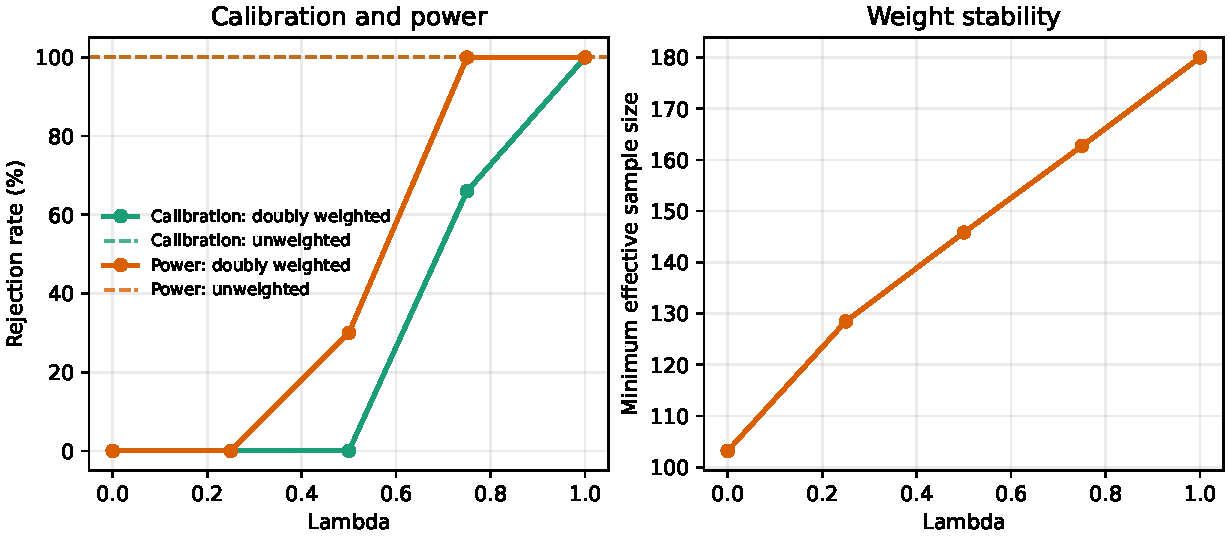
\includegraphics[width=0.98\linewidth]{figures/lambda_sensitivity_plot.pdf}
	\caption{Sensitivity to $\lambda$. Two-panel figure sharing the same x-axis ($\lambda$). Left panel (y-axis: rejection rate) shows calibration and power across $\lambda$ as solid lines for the doubly weighted mode, with horizontal dashed lines for the corresponding unweighted baseline. Right panel (y-axis: minimum effective sample size) tracks weight stability across the same $\lambda$ grid. Smaller $\lambda$ values correct weak-overlap bias more strongly but increase weight concentration. Larger values approach the unweighted regime.}
	\label{fig:lambda-sensitivity}
\end{figure}


\subsection{Permutation Resample Sensitivity}
\label{app:perm-sensitivity}

All permutation tests use $n_{\text{resamples}}$ Monte Carlo draws from the null distribution.
The main synthetic experiments use $n_{\text{resamples}} = 499$; the domain-classifier sensitivity
uses $999$; the second DGP uses $199$. These values were checked to ensure that increasing
$n_{\text{resamples}}$ would not materially change any reported figure or table.

The Monte Carlo standard error of a permutation p-value at a threshold $\alpha$ is
$\sqrt{\alpha(1-\alpha)/n_{\text{resamples}}}$ and the discrete step between
consecutive p-values is $\Delta = 1/(n_{\text{resamples}}+1)$.
With $n_{\text{resamples}} = 499$, $\text{SE}(p = 0.05) \approx 0.010$ and
$\Delta = 0.002$; the expected rejection rate under the exact null is
$4.8\%$ rather than $5\%$ (a $0.2$ percentage-point conservatism from discreteness).
With $n_{\text{resamples}} = 199$, the null rejection rate is $4.5\%$.

We simulated the ``flip rate'' --- the probability that a single trial's
reject/not-reject decision changes when using $n_{\text{resamples}}$ versus
$n_{\text{resamples}} = 9999$ (which approximates the exact test). Under the null,
the flip rate is $0.7\%$ for $n_{\text{resamples}} = 499$ and $1.3\%$ for
$n_{\text{resamples}} = 199$. Under the alternative, most p-values are at the
achievable floor ($1/500 = 0.002$), giving a flip rate of essentially zero.

The aggregate effect over $100$ independent trials (the standard experiment
size) is negligible. The standard deviation of the difference in reported
rejection rates between $n_{\text{resamples}} = 499$ and a near-exact test
is $0.009$; the probability that this difference exceeds $2$ percentage points
is approximately $6\%$, and the probability that it exceeds $5$ percentage
points is below $0.1\%$. For the second DGP ($40$ trials, $n_{\text{resamples}} = 199$)
these bounds are slightly wider but remain well within the uncertainty already
present from finite-repetition variability.

\sloppy

Build the manuscript from \path{research/papers/dw/}.

\begin{itemize}
\item Run \texttt{make} for the full PDF build.
\item Run \texttt{make figures} to refresh the plots.
\item Run \texttt{make tables} to rebuild the calibration table.
\end{itemize}

Generated artifacts are written to:

\begin{itemize}
\item \path{research/papers/dw/results/}
\item \path{research/papers/dw/figures/}
\item \path{research/papers/dw/tables/}
\end{itemize}

The experiments use the following settings:

\begin{itemize}
\item Shared settings: $100$ repetitions, $499$ permutation resamples per run, and balanced source-target sample sizes of $180$ for calibration, power, mode comparison, and lambda sensitivity.
\item Calibration: severity grid $0.0, 0.1, 0.2, 0.3, 0.4$ with fixed $\lambda = 0.5$.
\item Power: severity $0.25$ with shared-support effect-size grid $0.0, 0.15, 0.3, 0.45, 0.6$.
\item Mode comparison: contamination settings $(0.25, 0.0)$, $(0.0, 0.25)$, and $(0.25, 0.25)$ with $\lambda = 0.5$.
\item Lambda sensitivity: severity $0.25$, power effect size $0.4$, and $\lambda$ grid $0.0, 0.25, 0.5, 0.75, 1.0$.
\item Real-data workflow study: four mirrored tasks (HELOC, diabetes readmission, ACS income, and ACS public coverage); five-fold domain-classifier CV; at most $30{,}000$ source-train rows and $4{,}000$ held-out source plus $4{,}000$ target evaluation rows per task; $499$ permutation resamples per test; seed $123456$; default $\lambda = 0.5$.
\end{itemize}

The real-data workflow study reports predicted risk, model confidence, and prediction error from one source-trained model per task. The metadata JSON records the exact OpenML IDs, split rules, task sizes, script arguments, and package commit. \emph{Snapshot note:} committed \texttt{results/} and \texttt{figures/} in this revision are carried from \texttt{2f42d61}; \texttt{verify\_result\_metadata} reports them as pre-stale until the full pipeline is regenerated from the rebased branch (port to \texttt{samesame} 0.4.1 verified via smoke tests in \S\ref{app:domain-clf-sensitivity}). Regeneration via \texttt{make} is planned before submission and will refresh all hashes.

\subsection{Reproducibility Checklist}

\begin{itemize}
    \item All experiments use public datasets available through OpenML with pinned dataset IDs.
    \item Synthetic data is generated from reproducible random seeds.
    \item The full experiment pipeline is available in \texttt{research/papers/dw/scripts/} and executable via \texttt{make}.
    \item All result files include metadata recording the commit hash, script arguments, and input file checksums.
    \item Random seeds are explicitly recorded in each experiment script and incremented per repetition.
    \item Permutation inference uses 499 resamples; sensitivity to resample count is verified in \S\ref{app:perm-sensitivity}. The second DGP uses 199 resamples and the domain-classifier experiment uses 999; both are within the stable regime documented there.
    \item Domain classifiers use default hyperparameters unless otherwise noted.
\end{itemize}

\fussy
